\chapter{AAA model}

AAA controls who is permitted to access a network (Authenticate), what they can do while they are there (Authorize), and to audit what actions they performed while accessing the network (Accounting).

\section{Authentication}

\subsection{Local}

Local AAA Authentication uses the local usernames and passwords stored on a router. A drawback of the this method is that user accounts must be configured locally on each device, which does not scale well for large enterprise. The local authentication only serves as a backup method for if authentication servers are not available. 

\begin{itemize}
  \item Add usernames and passwords to the local router database for users that need administrative access to the router.
  \item Enable AAA globally on the router.
  \item Configure AAA parameters on the router.
  \item Confirm and troubleshoot the AAA configuration.  
\end{itemize}

\begin{sexylisting}{Local default authentication}
username ADMIN algorithm-type scrypt secret Str0ng5rPa55w0rd
username JR-ADMIN algorithm-type scrypt secret Str0ng5rPa55w0rd
aaa new-model
aaa authentication login default local-case
\end{sexylisting}

The above commands create two users ADMIN and JR-ADMIN, then uses local database to authenticate these users when they login the router (the last command). The \code{default} keyword means that the authentication method applies to all lines (console, vty, aux). Alternatively, you can name an authentication method  and assign it to a particular line.\\ 

\begin{sexylisting}{Local named authentication}
aaa authentication login SSH-LOGIN local-case
line vty 0 4
login authentication SSH-LOGIN
\end{sexylisting}

%The final portion of the \code{aaa authentication login} command identifies the type of methods that will be queried to authenticate the users, which is \code{local-case}. When a user attempts to log in, the first method listed is used. Cisco IOS software attempts the second authentication method only when there is no response or an error from the first method occurs. This process continues until no other authentication methods are available.\\
%
%The \code{aaa local authentication attempts max-fail} command locks the user account if the authentication fails. The locked out user account remains locked until it is manually cleared by an administrator using the \code{clear aaa local user lockout} privileged EXEC mode command. This command is different from \code{login delay} command, which introduces a delay between failed login attempts without locking the account.\\

To display a list of all locked-out users, use the \code{sh aaa local user lockout} command. To display the history of activities (attributes), use the \code{sh aaa user} command. The \code{sh aaa sessions} command can be used to show the unique ID of a session.

\subsection{Server-based}

\tableStart[\caption{TACACS+ and RADIUS protocols}\label{ACS}] {|p{5\xm}|p{5\xm}|} 
\head{TACACS+} & \head{RADIUS} \w
Separates authentication and authorization & Combines RADIUS authentication and authorization as one process.\w
Encrypts all communication & Encrypts only the password using MD5 \w
TCP port 49 & UDP port 1645 or 1812 for authentication, UDP port 1646 or 1813 for accounting\w
Multiprotocol support & Supports remote-access technologies, VoIP, 802.1X, and Session Initiation Protocol (SIP) \w
\tableEnd

Cisco Secure ACS for Windows Server is a single solution that offers AAA for both TACACS+ and RADIUS and is integrated to into Active Directory service. In this technology, Active Directory controller performs the authentication and authorization.

%There are three basic steps to configure server-based authentication:
%
%\begin{enumerate}
%\item \textbf{Username:} Create a username with encrypted password
%\item \textbf{Enable:} Globally enable AAA
%\item \textbf{Server:} Specify either TACACS+ or RADIUS server
%\item \textbf{Key:} 
%\item \textbf{Method list:} Configure the AAA authentication method list to refer to the TACACS+ or RADIUS server. For redundancy, it is possible to configure more than one server.
%\item \textbf{Applying:} Configure AAA authentication for console, or vty login to use the the newly configured AAA authentication method.
%\end{enumerate}




\begin{sexylisting}{Server-based authentication}
aaa new-models
username ADMIN algorithm-type scrypt secret Str0ng5rPa55w0rd

#STEP 2: TACACS+ server
tacacs server Server-T
  address ipv4 192.168.1.101
  single-connection
  key TACACS-Pa55w0rd

#STEP 2: RADIUS server 
radius server Server-R
  address ipv4 192.168.1.101 auth-port 1812 acct-port 1813
  key RADIUS-Pa55w0rd

aaa authentication login default group tacacs+ group radius local-case

line con 0
	login authentication default 
\end{sexylisting}

On TACACS+ or  Radius  server, you have to set up an entry as shown in figure \ref{RADIUSserver}. On router CLI, configure a corresponding entry with the server's address and the exact same encryption key with the server.\\

\begin{figure}[hbtp]
\caption{Add an entry for a router in a RADIUS server}\label{RADIUSserver}
\centering
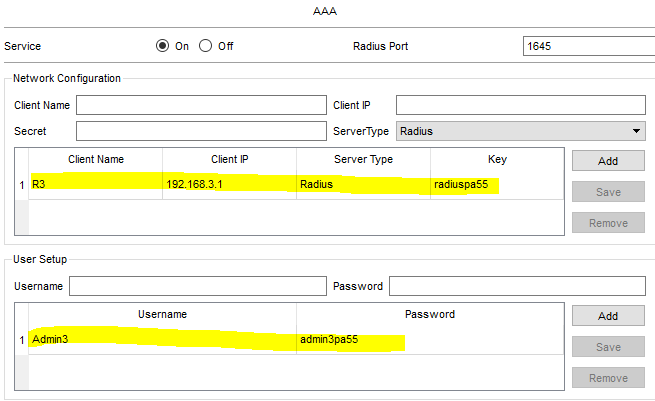
\includegraphics[scale=1]{pictures/RADIUSserver.PNG}
\end{figure}

%The \code{address ipv4} command allows the option to modify IPv4 address of the server, authentication port, and accounting port. The \code{key} command is used to configure the shared secret key, which must be exactly the same way on both the router and the server.\\

By default, TACACS+ establishes a new TCP session for every authorization request, which can lead to delays when users enter commands. To improve performance, Cisco Secure ACS supports persistent TCP sessions configured with the \code{single-connection} tacacs server configuration mode command. \\

We add AAA servers to the method list using the \code{group tacacs+} or \code{group radius} keywords. The above command configures a method list that first uses TACACS+ server for authentication. If TACACS+ server is unreachable, the RADIUS server takes over, and the last resort is local authentication (case-sensitive).

\section{Authorization and Accounting (server-based only)}

When AAA authorization is not enabled, all users are allowed full access. After authentication is started, the default changes to allow no access. This means that the administrator must create an administrative user before authorization is enabled. Failure to do so immediately locks the administrator out of the system.

\begin{sexylisting}{Authorization}
aaa new-models
username ADMIN algorithm-type scrypt secret Str0ng5rPa55w0rd
aaa authorization exec default group tacacs+
line vty 0 4
	authorization exec default
\end{sexylisting}%

Instead of \code{exec} (For starting an exec mode), you can specify another  types of commands or services such as \code{network} (network services such as PPP), or \code{commands <level>} (exec commands).

\begin{sexylisting}{Accounting Configuration}
aaa account exec default start-stop group tacacs+
\end{sexylisting}

The following three parameters are commonly used aaa accounting keywords:

\begin{itemize}
\item \code{network} - Runs accounting for all network-related service requests, including PPP.
\item \code{exec} - Runs accounting for the EXEC shell session.
\item \code{connection} - Runs accounting on all outbound connections such as SSH and Telnet.
\end{itemize}

Next, the record type, or trigger, is configured. The trigger specifies what actions cause accounting records to be updated. Possible triggers include:

\begin{itemize}
\item \code{start-stop} - Sends a "start" accounting notice at the beginning of a process and a "stop" accounting notice at the end of a process.
\item \code{stop-only} - Sends a "stop" accounting record for all cases including authentication failures.
\item \code{none} - Disables accounting services on a line or interface.
\end{itemize}
    

\section{802.1X Port-Based Authentication}

\subsection{Operation}

The IEEE 802.1X standard defines a port-based access control and authentication protocol that restricts unauthorized devices from connecting to a LAN through publicly accessible switch ports. Figure \ref{802.1X} shows that with 802.1X port-based authentication roles:

\begin{itemize}
\item \textbf{Supplicants} are users' devices, which must have 802.1X-compliant client software. 
\item \textbf{Authenticators} are usually switches, which act as intermediary (proxy) between the supplicants and the authentication server. It uses a RADIUS software agent, which encapsulates and de-encapsulates the EAP frames to interact with the authentication server.
\item \textbf{The authentication server} authenticates the client and notifies the switch to enable or disable access. Because the switch acts as the proxy, the authentication service is transparent to the client.
\end{itemize}

\begin{figure}[hbtp]
\caption{802.1X roles}\label{802.1X}
\centering
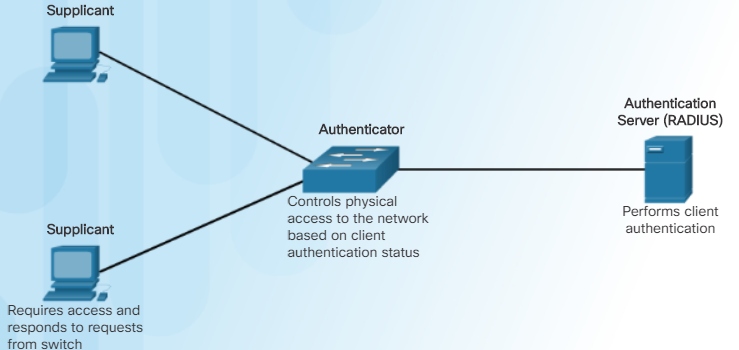
\includegraphics[scale=0.7]{pictures/8021X.PNG}
\end{figure}


While in \emph{unauthorized state}, the port disallows all ingress and egress traffic except for 802.1X protocol packets. When a client is successfully authenticated, the port transitions to the \emph{authorized state}, allowing all traffic for the client to flow normally. When a client logs out, or the link state of the switch port changes from up to down, the switch port transitions to the unauthorized state.\\


\subsection{Configuration}

The following commands show a scenario where a PC is attached to F0/1 on the switch and the device is getting authenticated via 802.1X with a RADIUS server.

\begin{sexylisting}{802.1X configuration}
aaa new-models
radius server Server-R
  address ipv4 192.168.1.101 auth-port 1812 acct-port 1813
  key RADIUS-Pa55w0rd
  exit
aaa authentication dot1x default group radius
dot1x system-auth-control

interface f0/1
  sw mode access
  authentication port-control auto
  dot1x pae authenticator
  exit
\end{sexylisting}

We create an 802.1X port-based authentication method list using the \code{dot1x} key word. In interface configuration mode, the \code{authentication port-control auto} command enables 802.1X authentication. This command has two more options, \code{force-authorized} and \code{force-unauthorize}, which disable 802.1X authentication. The first option causes the port to remain authorized and allow normal traffic, while the second puts the port in unauthorized state and lock all authentication.